\subsection{Разложение рисунка}
По аналогии с разложением комплексной параметрической функции, можно найти разложение в ряд Фурье для функции, график которой представляет из себя интересующий нас рисунок. 

Нам подойдет рисунок в векторном формате, который состоит из одной замкнутой линии. Она не должна иметь толщины. В редакторе CoralDraw для этого существует параметр \textit{сверхтонкий абрис}. 

\begin{figure}[ht!]
    \centering
    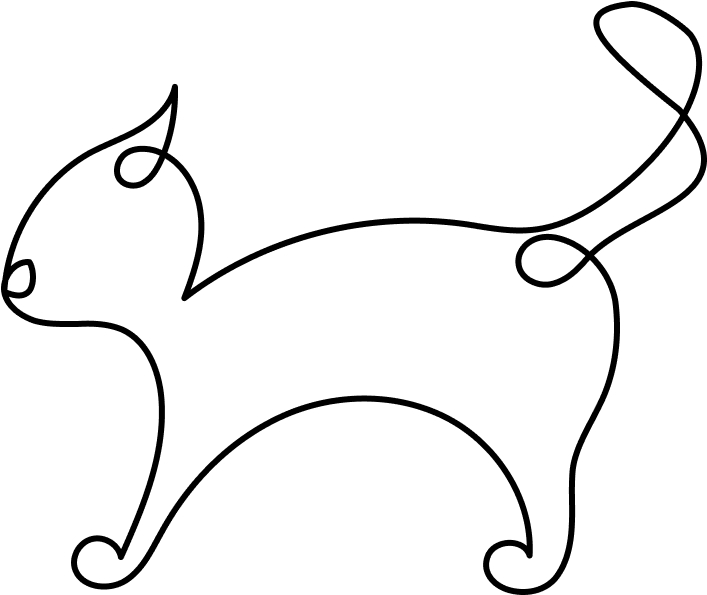
\includegraphics[width=0.5\textwidth]{./media/cat.jpg}
    \caption{Рисунок, который будет раскладывать}
    \label{fig:cat}
\end{figure}

Возьмем рисунок с котиком. Для того, чтобы \textit{достать} параметрический график из svg файла можно использовать библиотеку \texttt{svg.path} и ее функцию \texttt{parse\_path}. 

\begin{lstlisting}[style=python_white, caption={Получение параметрической функции рисунка}, label=lst:parametric_function]
path = svg.path.parse_path(spline)
path_func = np.vectorize(lambda t: path.point(t) * scale)
\end{lstlisting}

В результате работы кода (см. листинг~\ref{lst:parametric_function}) получаем параметрическую функцию $path\_func(t)$, где $t \in [0, 1]$, 
которая будет возвращать точку на комплексной плоскости. 

Теперь данную функцию можно разложить в ряд Фурье на отрезке $[0, 1]$ с помощью функции \texttt{fourier\_exp} (см. листинг~\ref{lst:fourier_cat}). 
В результате работы этой функции получим набор коэффициентов $c_n$, которые являются коэффициентами искомого разложения рисунка. 

Для проверки полученного результата можно построить \textit{графики} полученных функций (количество коэффициентов $N=20$) (см рис. \ref{fig:cat_plot}). 
Видим, что оба графика крайне похожи друг на друга. Это значит, что разложение Фурье корректно применилось для нашего рисунка. 

\begin{figure}[ht!]
    \centering
    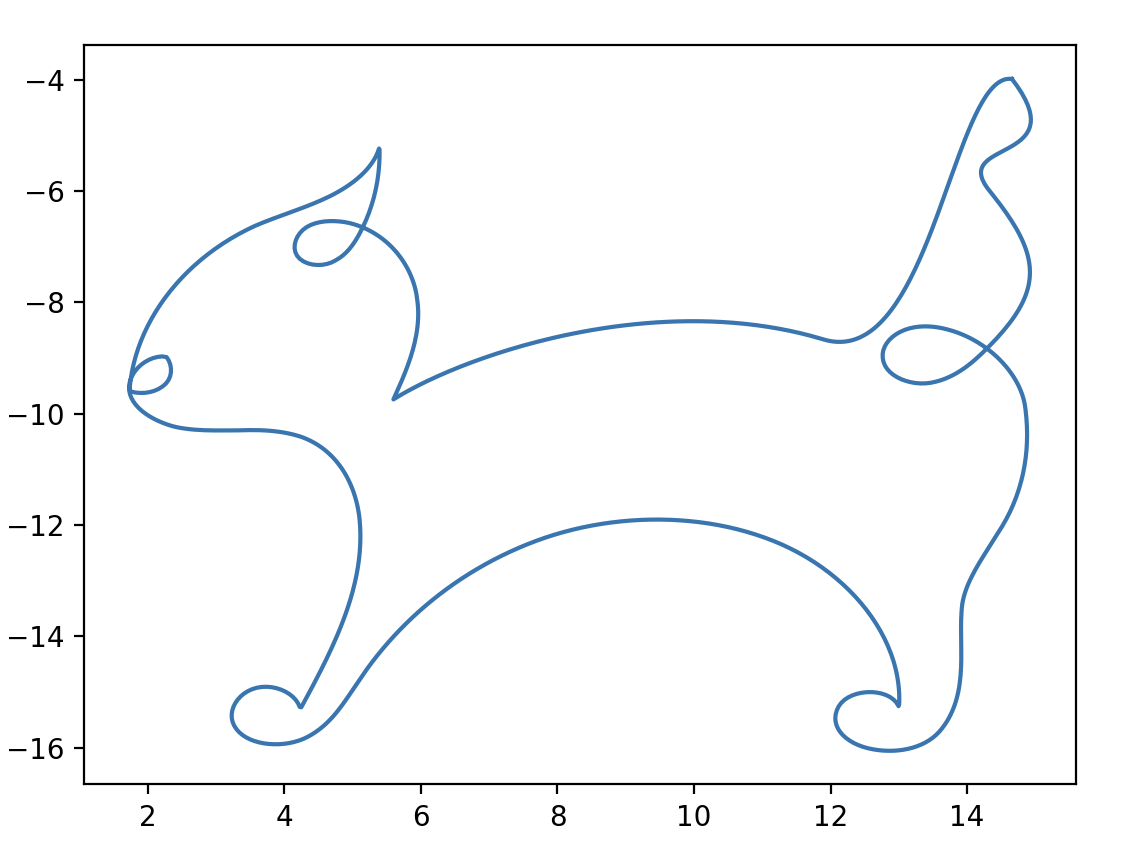
\includegraphics[width=0.49\textwidth]{./media/cat_func.png}
    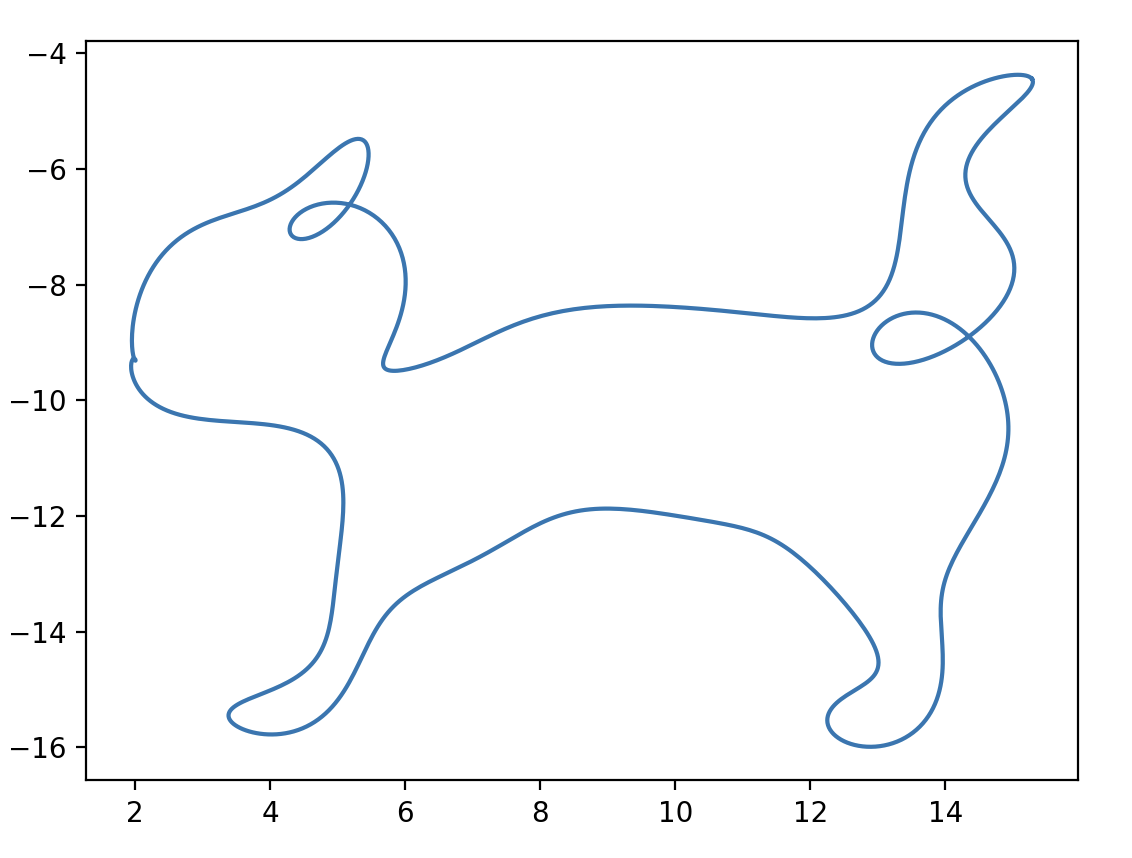
\includegraphics[width=0.49\textwidth]{./media/cat_fourier.png}
    \caption[]{Исходный рисунок и рисунок после разложения Фурье ($N = 20$)}
    \label{fig:cat_plot}
\end{figure}

\subsection{Вращаем векторы}
Теперь разберемся с тем, как можно представить полученные коэффициенты разложения с виде движущихся с целой частотой относительно друг друга векторов. 

Из разложения (см. формулу \ref{eq:fourier_exp}) мы имеем слагаемые вида:
\begin{equation}
    c_i\cdot e^{i\omega_it}
    \notag
\end{equation}
Каждый из коэффициентов $c_i$ имеет комплексное значение, при этом $i$ определяет частоту вращения вектора (об/ceк, если $i < 0$, то вращение в другую сторону).

Для определения радиуса круга с номером (и частотой вращения) $i$ можно воспользоваться следующей формулой: 
\begin{equation}
    r = \sqrt{Re(c_i)^2 + Im(c_i)^2}
\end{equation}
Это будет радиус окружности, внутри которой вращается вектор. 

Начальное положение вектора будем задавать как часть дуги (от 0 до 1), на которую должен \textit{указывать} вектор. Обозначим это значение $\phi$
Найти его можно следующим образом: 
\begin{equation}
    \phi = \begin{cases}
        \frac{atan2(-Im(c_i),~Re(c_i))}{2\pi} & atan2(Im(c_i), Re(c_i)) > 0\\
        \frac{atan2(-Im(c_i),~Re(c_i)) + 2\pi}{2\pi} & atan2(Im(c_i), Re(c_i)) <= 0
    \end{cases}
\end{equation}
После мнимой части стоит минус для того, чтобы рисунок не был перевернутым. 

Теперь, когда у нас есть все нужные значения (частоты вращения векторов, длины векторов, начальные положения), мы можем перейти к отрисовке. 

\subsection{Отрисовка графики}

Основной единицей в программе являются объект класса \texttt{RotatingCircle} (см. листинг~\ref{lst:rotating_circle}), который наследован от класса \texttt{Circle} -- вращающаяся окружность. 
В нем добавлены поля, хранящие окружность, по орбите которой она вращается, частота вращения и позиции \textit{точки} на этой окружности. 

Кроме того, добавлены классы \texttt{VectorInCircle} и \texttt{DotOnCircle}, наследованные от классов 
\texttt{Arrow} и \texttt{Dot} соответственно. Они нужны лишь для визуализации соответствующих элементов. 

Все \textit{действие} основано на обновлении точек на окружностях, и, соответственно, центов окружностей, которые привязных к этим точках.

Функция \texttt{rotating\_circle\_updater} изменяет положение точки на окружности, \texttt{dot\_on\_circle\_updater} -- перемещает точку по окружности, \texttt{vector\_in\_circle\_updater} -- перемещает начало вектора в центр окружности, в которой он расположен и конец вектора к точке на этой же окружности. 

Таким образом, изменение положения центра окружности и положения точки на ней ведет к изменений положения всех элементов. 

В основном методе рассчитываются коэффициенты $c_i$ и создаются \textit{вложенные} окружности (родителем каждой следующей окружности является предыдущая), центр которых привязывается к точке на родительской окружности. 
Таким образом создается зависимость положения дочерних окружностей от родительских. 

В результате получаем анимацию с отрисовкой исходного рисунка (\href{https://drive.google.com/file/d/1bMOGz81cHuQbmYTLcZKFB8C2WC-LNEim/view?usp=share_link}{ссылка}):  

Так же можно посмотреть на анимации при различных значениях $N$ (\href{https://drive.google.com/drive/folders/1dmXw8v6x5eByshXMqzxIWHGvhgOteTDo?usp=share_link}{ссылка}). 

Исходный код находится в приложении \ref{appendix:appendixB}. 

\begin{figure}[ht!]
    \centering
    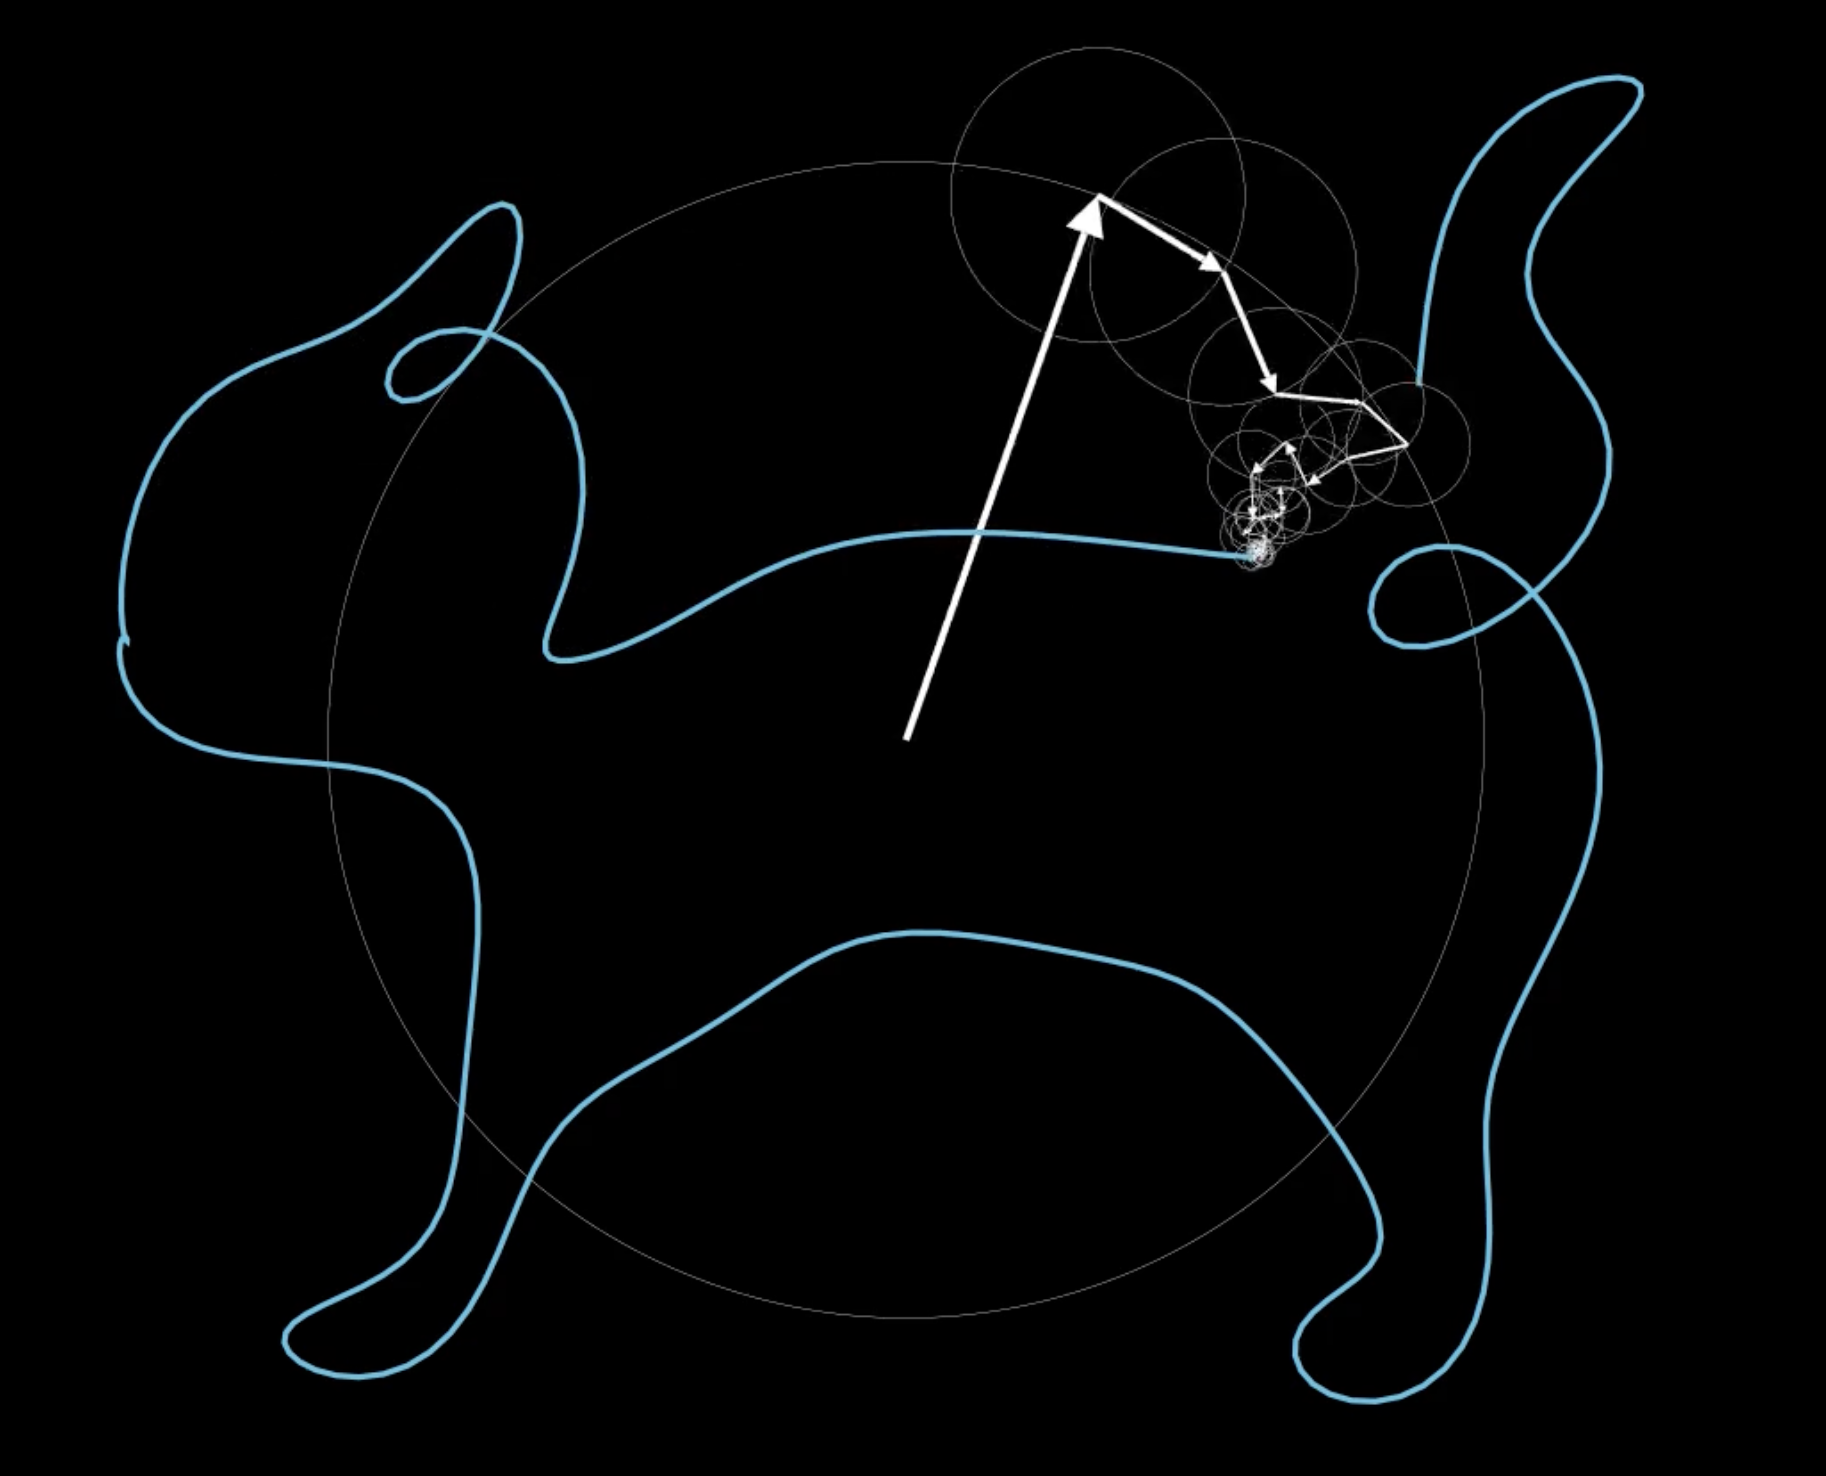
\includegraphics[width=0.6\textwidth]{./media/cat_animation.png}
    \label{fig:cat_animation}
    \caption{Стоп-кадр из анимации}
\end{figure}
Полученный рисунок полностью совпадает с тем, что был получен из частичной сумму ряда Фурье (см. рис.~\ref{fig:cat_plot}).